% -----------------------------------------------------------------------
% --- DOCUMENT ---
% -----------------------------------------------------------------------
\documentclass[11pt, a4paper, french, twoside]{article}

% -----------------------------------------------------------------------
% --- PACKAGE ---
% -----------------------------------------------------------------------
\usepackage[french]{babel}

% Font
\usepackage[utf8]{inputenc}
\usepackage[T1]{fontenc}

% Marge du document
\usepackage[top=3.5cm,
	bottom=3cm,
	left=2cm,
	right=2cm,
	footskip=1.5cm,
	headheight=1.5cm,
	headsep=0.9cm]{geometry}

% Gérer les positionnement d'images
\usepackage{float}

% Import de fichier externe
\usepackage{graphicx}

% Mise en forme des URL
\usepackage{url}

% Informations sur un document compilé en PDF et les liens externes / internes
\usepackage{hyperref}

% Pour les entêtes
\usepackage{fancyhdr}

% -----------------------------------------------------------------------
% --- INFORMATION SUR LE DOCUMENT
% -----------------------------------------------------------------------

% Information sur le document
\hypersetup{
	pdfauthor = {Kirushnapillai Sathiya, Monteverde Mathieu, Zucca Michela},                    % Auteurs
	pdftitle = {Project Cours Scala},                         % Titre du document
	pdfsubject = {Rapport},                % Sujet
	pdfstartview={FitH}}                            % ajuste la page à la largueur de l'écran

% -----------------------------------------------------------------------
% --- EN-TETE ET PIED DE PAGE ---
% -----------------------------------------------------------------------
\pagestyle{fancy}
\fancyhf{} % Supprime les entetes et pieds de page existants

\fancyhead[LE,RO]{Rapport\\}
\fancyhead[LO]{
\includegraphics[width=4cm]{images/logo_heig.png}}
\fancyfoot[LE,RO]{\thepage{}}
\fancyfoot[RE]{Kirushnapillai Sathiya, Monteverde Mathieu, Zucca Michela}
\fancyfoot[LO]{Project Cours Scala}
\renewcommand{\footrulewidth}{1pt}


\title{Project Cours Scala \\ Rapport}
\author{Kirushnapillai Sathiya, Monteverde Mathieu, Zucca Michela}
\date{2018}


\begin{document}
	\selectlanguage{french}
	\graphicspath{ {images/} }
	
	% Espacement entre les lignes
	\newcommand{\HRule}{\rule{\linewidth}{0.5mm}}
	
	% Page de garde
	\begin{titlepage}
    \begin{center}

	 \vspace{0.5cm}
     {\fontsize{1.5cm}{1.8cm} \bf Project Cours Scala}\par
     \vspace{0.5cm}
     {\fontsize{0.9cm}{1.3cm} \selectfont Description du projet}\par
     \vspace{3cm}
     \vfill
        
        % Author and supervisor
        \begin{minipage}{0.4\textwidth}
        	\begin{flushleft} \large
        		\textbf{Auteurs:}\\
        		\textsc{Kirushnapillai} Sathiya \\
        		\textsc{Monteverde} Mathieu \\
        		\textsc{Zucca} Michela
        	\end{flushleft}
        \end{minipage}
        \begin{minipage}{0.4\textwidth}
            \begin{flushright} \large
                \textbf{Professeur:} \\
                \textsc{Fatemi} Nastaran \\
            \end{flushright}
        \end{minipage}
    
        \vfill
    \begin{minipage}{0.4\textwidth}
    	\begin{flushleft} \large
       		
\includegraphics[width=5cm]{images/logo_heig.png}
        \end{flushleft}

	\end{minipage}
	\begin{minipage}{0.4\textwidth}
	    \begin{flushright}
			
\includegraphics[width=5cm]{images/logo-hes-so.jpg}
		\end{flushright}
	\end{minipage}


        % Bottom of the page
        \today
        
    \end{center}
\end{titlepage}

	
	% Recommencer la numérotation des pages à "1"
	\setcounter{page}{1}
	\newpage
	
	% Espacement des paragraphes
	\setlength{\parskip}{0.2cm}
	
	\section{Contexte}
	\label{sec:contexte}
		Ce projet s'effectue dans le cadre du cours SCALA 2018. L'objectif est de réaliser une application Web en utilisant la technologie Scala Play pour le back-end et Slick pour la base de données. Le choix de la technologie front-end est libre.
		
	\section{Cahier des charges initial}
	\label{sec:description}
	
		\subsection{Buts}
		\label{subsec:buts}
		L'idée de ce projet est de proposer une plateforme Web permettant de partager des événements avec ses utilisateurs. Un utilisateur inscrit au préalable (subsequenceset faisant partie d'une organisation) pourra enregistrer des événements (par exemple un concert, une journée portes-ouvertes, un festival, etc.) en spécifiant des informations comme par exemple la localisation (coordonnées GPS ou adresse), une description, une ou plusieurs dates et des horaires.
		
		Un visiteur du site pourra ensuite rechercher les événements situés dans une certaines zone (par exemple dans un rayon de 10km autour de Lausanne) en spécifiant différents paramètres comme la date ou l'heure. 
		
		Le but est d'offrir un service indépendant de tout réseau social permettant à ses utilisateurs de trouver facilement des événements culturels ou festifs autour d'eux. 
		
		Une organisation est une entité (entreprise, commune, association, etc.) qui peut-être certifiée. Cela permet un certain contrôle sur le type d'événements qui sont créées (éviter les faux événements, les fêtes d'anniversaire, etc.).
	
	\section{Fonctionnalités}
	\label{sec:fonctionnalites}
		Cette section liste les fonctionnalités qu'offrira la plateforme pour les différents acteurs. 
		
		\subsection{Priorités}
		\label{subsec:priorites}
		
		\begin{itemize}
			\item 1 - Obligatoire
			\item 2 - Obligatoire si aucun retard dû à l'apprentissage
			\item 3 - Optionnel ou futur
		\end{itemize}
		
		\subsection{Visiteur}
		\label{subsec:visiteur}
			Un utilisateur non-authentifié de l'application Web pourra: 
			
			\subsubsection{Affichage et tri d'événements}
			\label{subsubsec:affichage_tri_evenements}
			
				\begin{itemize}
					\item Voir une liste d'événements [1]
					\item Filtrer une liste d'événements par date [1]
						\begin{itemize}
							\item Choisir une date exacte [1]
							\item Choisir une plage avec date de début et date de fin [1]
						\end{itemize}
					\item Filtrer une liste d'événements par lieu géographique [1]
						\begin{itemize}
							\item Choisir une ville départ [1]
							\item Choisir un rayon de recherche autour de cette ville [2]
						\end{itemize}
					\item Rechercher un événement [1]
						\begin{itemize}
							\item Recherche par nom d'événement [1]
							\item Recherche par organisation [1]
						\end{itemize}
					\item Filtrer une liste d'événement par thème [1]
					\item Voir le détail d'un événement [1] 
				\end{itemize}
			
			\subsubsection{Inscription}
			\label{subsubsec:inscription}
			
				\begin{itemize}
					\item Créer un compte sur la plateforme [1]
						\begin{itemize}
							\item E-mail
							\item Mot de passe
							\item Nom d'utilisateur
							\item Prénom
							\item Nom de famille
						\end{itemize}
					\item Envoi d'un e-mail de confirmation à l'inscription [3]
				\end{itemize}
		
		\subsection{Utilisateur inscrit}
		\label{subsec:utilisateur_inscrit}
			Un utilisateur authentifié pourra:
			
			\subsubsection{Profil}
			\label{subsubsec:profil}
			
				\begin{itemize}
					\item Afficher son profil [1]
					\item Modifier les informations de son profil [2]
					\item Supprimer son profil [3]
					\item Lier son profil à son compte Facebook [3]
				\end{itemize}
			
			\subsubsection{Organisations}
			\label{subsubsec:organisations}
			
				\begin{itemize}
					\item Créer une organisation [1]
						\begin{itemize}
							\item Spécifer le type d'organisation (Entrprise, association, ville, etc.)
							\item Spécifier le nom de l'organisation
							\item Spécifier l'adresse
							\item D'autres informations si nécessaire
						\end{itemize}
					\item Afficher les informations des organisations dont il fait partie [1]
					\item Ajouter des utilisateurs à une organisation [1]
					\item Modifier les informations des organisations dont il fait partie [2]
					\item Supprimer une organisation [3]
					\item Lier l'organisation à une page Facebook [3]
				\end{itemize}
			
			\subsubsection{Evénements}
			\label{subsubsec:evenements}
				\begin{itemize}
					\item Créer un événement au nom d'une organisation dont il fait partie [1]
						\begin{itemize}
							\item Titre
							\item Description
							\item Prix
							\item Lieu (Adresse ou coordonées géographiques)
							\item Date de début
							\item Date de fin
							\item Horaires
							\item Organisation
							\item Thèmes de l'événement
						\end{itemize}
					\item Modifier un événement d'une organisation dont il fait partie [1]
					\item Supprimer un événement d'une organisation dont il fait partie [2]
					\item Marquer un événement comme appartenant à ses favoris [1]
					\item Afficher ses événements favoris [1]
					\item Retirer un événement de ses favoris [1]
					\item Copier le contenu depuis un événement Facebook (de son profile Facebook ou d'une page qu'il gère) [3]
				\end{itemize}
			
			\subsubsection{Commentaires}
			\label{subsubsec:commentaires}
			
				\begin{itemize}
					\item Publier un commentaire sur un événement [3]
					\item Supprimer un commentaire sur un événement [3]
				\end{itemize}
			
			
			\subsubsection{Thèmes}
			\label{subsubsec:themes}
			
			\begin{itemize}
				\item Ajouter des thèmes comme centre d'intérêt [1]
				\item Modifier ses centres d'intérêt [1]
			\end{itemize}
		
			\subsubsection{Notifications}
			\label{subsubsec:notifications}
			
				\begin{itemize}
					\item Voir une liste de notifications signalant les événements conformes à ces intérêts lorsqu'il se connecte [2]
					\item recevoir un e-mail de notification [3] 
				\end{itemize}
			
	\section{Implémentation}
		\subsection{Structure de la base de données}
		\label{subsec:structure}
			La figure \ref{fig:er} illustre le schéma entité-relation de la base de données du projet. L'application comporte des utilisateurs (User), des organisations (Organization) et des évenements (Event). Pour chaque entité, les opérations de base (CRUD) seront fournies : Afficher, créer, modifier et supprimer. Cependant, seuls les utilisateurs liés à une organisation peuvent créer, modifier et supprimer des événements.
			
			Pour cette première ébauche, chaque événement possède un ou plusieurs thèmes (Theme) qui permettront aux visiteurs de filtrer leurs recherches. Les thèmes permettent également aux utilisateurs inscrits d'être notifié d'un nouvel événement selon leurs préférences (Ce dernier point est pour l'instant optionnel).
			
			Et enfin, l'application permettra également aux utilisateurs inscrits de commenter un événement.
			
			\begin{figure}[h]
				\centering
				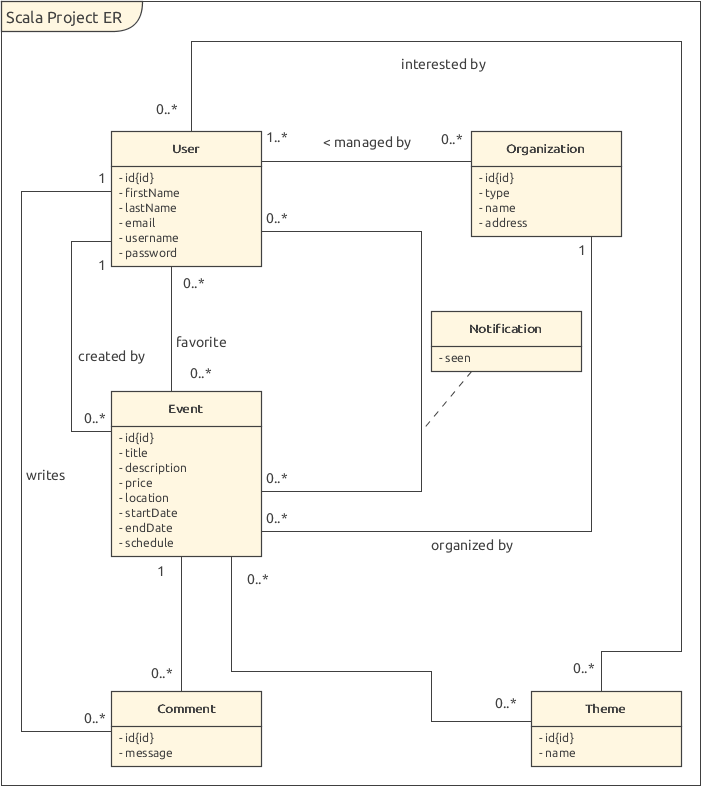
\includegraphics[width=0.8\linewidth]{images/project_ER.png}
				\caption{Schéma entité-relation de la base de données}
				\label{fig:er}
			\end{figure}
		
		\subsection{Fonctionnalités implémentées}
		\label{subsec:fonctionnalites_implementees}
		
			Cette section présente les fonctionnalités du cahier des charges qui ont été implémentées.
		
			\subsubsection{Affichage et tri d'événements}
			\label{subsubsec:affichage_tri_evenements}
			
			\begin{itemize}
				\item Voir une liste d'événements
				\item Filtrer une liste d'événements par date
				\begin{itemize}
					\item Choisir une date exacte
					\item Choisir une plage avec date de début et date de fin
				\end{itemize}
				\item Filtrer une liste d'événements par lieu géographique
				\begin{itemize}
					\item Choisir une ville départ
				\end{itemize}
				\item Voir le détail d'un événement
			\end{itemize}
		
			\subsubsection{Inscription}
				\begin{itemize}
					\item Créer un compte sur la plateforme
				\end{itemize}
			
			\subsubsection{Profil}
				\begin{itemize}
					\item Afficher son profil
					\item Modifier les informations de son profil
				\end{itemize}
			
			\subsubsection{Organisations}
				\begin{itemize}
					\item Créer une organisation
						\begin{itemize}
							\item Spécifier le type
							\item Spécifier le nom
							\item Spécifier l'adresse
						\end{itemize}
					\item Afficher les informations des organisations dont un utilisateur connecté fait partie
				\end{itemize}
			
			\subsubsection{Evénements}
				\begin{itemize}
					\item Créer un événement au nom d'une organisation dont l'utilisateur connecté fait partie
					\begin{itemize}
						\item Titre
						\item Description
						\item Prix
						\item Lieu (Adresse ou coordonées géographiques)
						\item Date de début
						\item Date de fin
						\item Horaires
						\item Organisation
					\end{itemize}
					\item Modifier un événement d'une organisation dont l'utilisateur connecté fait partie
					\item Supprimer un événement d'une organisation dont l'utilisateur connecté fait partie
					\item Marquer un événement comme appartenant aux favoris de  l'utilisateur connecté 
				\end{itemize}
		
			\subsubsection{Thèmes}
			
				\begin{itemize}
					\item Ajouter des thèmes comme centre d'intérêt
					\item Modifier ses centres d'intérêt
				\end{itemize}
	
	\section{Difficultés rencontrées}
		\subsection{Formulaires}
			Notre application dispose de nombreux formulaires qui sont indispensables à son bon fonctionnement (inscription, connexion, création d'événements). Une des difficultées rencontrées était de gérer la validation des formulaires et leur affichage de manière évolutive. 
			
			Pour ce faire nous avons étudié la documentation du framework Scala Play sur la gestion des formulaires. Cela nous a pris beaucoup de temps, mais comme cela est visible dans notre code source, le résultat en valait la peine, car cela permet de valider chaque soumission de formulaire en le comparant à un modèle pré-défini sans avoir à vérifier chaque champ à la main. 
			
			Cela nous a quand même pris un temps certain pour comprendre comment le faire, comme avec toute nouvelle technologie.
			
		\subsection{Apprentissage de la technologie}
			Scala Play Framework est un framework très puissant et très utile pour créer des applications Web ou des APIs REST. Cependant sa courbe d'apprentissage nous a semblé très élevée en début de projet. Il nous a fallu beaucoup de lecture et de temps pour comprendre correctement les concepts du framework (ou du langage Scala que nous avons découvert avec ce projet) tels que la gestion des requêtes asynchrones avec \textit{Async}, \textit{Future} \textit{Map} et la validation des formulaires.
			
	\section{Conclusion}
		Nous sommes globalement satisfait de ce projet et de la façon dont nous avons géré le développement. Nous n'avons pas implémenté toutes les fonctionnalités du cahier des charges, mais la majorité des fonctionnalités prioritaires ont été fournies. Etant donné le temps à disposition pour ce projet et la difficulté d'apprentissage du framework Play (comme avec tout framework aussi complet), nous pensons avoir atteint les objectifs de ce travail. 
		
\end{document}
